\setlength{\headheight}{13.59999pt}

This chapter is concerned with the method we have used to create semi-analytic models of planet wakes that encompass both the linear and non-linear disk response due to a perturbing planet as described in the previous chapter. 
This work builds on that presented in \citet{bollati2021} and so we will be predominantly concerned with the differences from their analysis.
However we aim to provide enough detail to be understandable without having read the aforementioned paper.

\section{Wakeflow: A Python Package For Semi-Analytic Models of Planet Wakes} \label{sec:JOSS}

This section has been submitted to the Journal of Open Source Science and is currently in review. The preprint is publicly available here: \url{github.com/TomHilder/wakeflow/blob/master/paper/paper.md}

\subsubsection{Summary}

\textsc{wakeflow} is a Python package for generating semi-analytic models of the perturbations induced by planets embedded in gaseous circumstellar disks. 
These perturbationstake the form of a spiral shock wave \citep{ogilvie2002}, and are often called a "planet wake" in analogy with that produced by a boat in a lake.

\subsubsection{Statement of Need}

Detecting newly formed planets embedded in their disk is a challenging problem in the field of planet formation. 
A major area of progress in recent years is the detection of planets by the gravitationally induced disturbance in their host disks. 
This disturbance, caused by the planet wake, manifests as a deviation in velocity from the bulk flow which may be measured through the Doppler shift of molecular lines \citep[eg.][]{perez2015, pinte2018a}. 
Such kinematic observations have been accurately reproduced through 3D fluid simulations of the planet-disk interaction, allowing for the inference of planet and disk properties \citep{pinte2018a, pinte2019}. 
However, these studies are computationally expensive.

\textsc{wakeflow} eases this computational cost by applying the theory of planet wake generation and propagation \citep{goldreich1979,goodman2001,rafikov2002a,bollati2021}to create semi-analytic models of planet wakes. 
\textsc{wakeflow} models are readily created in less than a minute on a modern laptop, as opposed to the hours of supercomputer time needed for 3D hydrodynamical simulations. 
The relatively low computational cost of \textsc{wakeflow}means that researchers can get an idea of whether planet-disk interactionscan explain their observations, and the disk and planet parameters needed, beforespending computer time on more detailed simulations.

\textsc{wakeflow} can interface with the radiative transfer code  \textsc{mcfost} \citep{pinte2006,pinte2009} in order to create synthetic observations of the semi-analytic models for direct comparison with observed continuum or line emission.

\textsc{wakeflow} is partially adapted from a previous Python code also written by us called \textsc{analytical\_kinks} \citep{bollati2021a}. 
\textsc{wakeflow} is intended to be a more complete, versatile and easy to use version of that code, and it obeys standard Python packaging conventions.
In addition, \textsc{wakeflow} can directly interface with \textsc{mcfost} while \textsc{analytical\_kinks} cannot.
At the time of writing, no other open source software packages exist to generate the perturbations induced by an embedded planet in a circumstellar disk using the semi-analytic theory of planet wakes.

Existing scientific publications focusing on detecting the kinematic signatures of planets that have used \textsc{wakeflow} or its predecessor \textsc{analytical\_kinks} include \citet{bollati2021}, \citet{calcino2022}, \citet{teague2022}, \citeauthor{garginreview} (in review) and \citeauthor{fasanoinprep.} (in prep.).

\subsubsection{Acknowledgements}

\textsc{wakeflow} relies on the following scientific Python packages: \textsc{NumPy} \citep{harris2020}, \textsc{matplotlib} \citep{hunter2007}, \textsc{SciPy} \citep{virtanen2020} and \textsc{Astropy} \citep{astropycollaboration2022}.

\section{Semi-Analytic Solution Algorithm}

As stated in the previous section, \textsc{wakeflow}

Outline the wakeflow algorithm for generating a model:
\begin{enumerate}
    \item Generate grid geometry. Interface with \textsc{mcfost if desired}.
    \item Calculate the unperturbed disk.
    \item Read in linear perturbations, scale, interpolate onto global grid geometry interpreting $y$ as an arc length in $\phi$. Mapped onto an annulus. Annulus is an update, more honestly displays results from shearing sheet approximation, minimises discontinuity in solution. Also, it is perfectly acceptable to extend the box vertically further since it is the position of the Lindblad resonances that matter ultimately for the linear regime not the planet itself (sort of).
    \item Extract initial conditions using \textbf{exact} transformations instead of approximate ones in \citet{bollati2021} to minimise discontinuity in solution.
    \item Solve Burger's equation until $t_{\rm f}=300$ using vectorised Godunov solver and adaptive time stepping.
    \item Get $\chi(r,\phi)$. Transformations are vectorised and the whole solution is interpolated in one go. Asymptotic regime and planet annulus are masked.
    \item Perturbations are calculated from $\chi$ using updated velocity mapping
\end{enumerate}

\section{Theoretical and Numerical Considerations} 

\note{Add something about how we are basically going into more detail for the steps in the algorithm and explaining the specific applications of or improvements to the stuff that been done before.}

\subsection{Unperturbed Disk Structure} \label{sec:diskstruct}

Here we outline the unperturbed disk model used in \textsc{wakeflow} onto which the perturbations are added.

\subsubsection{Temperature}

We assume that the sound speed $c$ obeys a simple radial power law 
\begin{align}
    c \propto r^{-q},
\end{align}
where $q$ is some real number. Thus the disk temperature scales as 
\begin{align}
    T \propto c^2 \propto r^{-2q}.
\end{align}
The constant of proportionality for these relations in determined by the user specified value of the disk aspect ratio $H/r$ at $r=r_{\rm ref}$

\subsubsection{Density}

We use a density structure derived by assuming that the disk is in vertical hydrostatic equilibrium \citep{pringle1981}, but unlike in \ref{eq:vertical_rho} we will not assume that $z\ll r$.
The density $\rho$ is given by 
\begin{align}
    \rho(r,z) \propto \left( \frac{r}{r_{\rm ref}} \right)^{-p} \exp{\left( \frac{G M_\star}{c^2} \left[ \frac{1}{\sqrt{r^2 + z^2}} - \frac{1}{r} \right] \right)},
\end{align}
where $p$ is some real number. 
The constant of proportionality is set directly by the user, or calculated by \textsc{mcfost} based on the total gas mass.

Very commonly the density profile is parameterised in terms of the surface density $\Sigma$, not the actual density $\rho$ as above.
If the surface density is parameterised as $\Sigma \propto r^{-\delta}$ where $\delta$ is some real number, then equation \ref{eq:surf_dens_to_dens} gives the approximate relation 
\begin{align}
    p \simeq \frac{3}{2} - q + \delta,
\end{align}
which can be used to convert between density parameterisations.
This conversion is only approximate in our context, since is does assume that $z \ll r$ and our density profile does not.
However this turns out not to matter since $\delta$ will only show up in the $t(r)$ mapping which we will assume is the same for all $z$.

\subsubsection{Velocities}

The radial and vertical motions in the unperturbed disk are set to zero. 
The rotation is derived assuming radial force balance \citep[eg.][]{nelson2013} and is given by 
\begin{align}
    \Omega(r,z) = \Omega_{\rm K} \left[ - \left(p + 2q\right) \left( \frac{H}{r} \right)^2 + \left( 1-2q \right) + \frac{2qr}{\sqrt{r^2 + z^2}}\right]^{1/2},
\end{align}
where $\Omega_{\rm K}$ is as defined in equation \ref{eq:point_pot}.

\subsection{Transformations}

\note{Something about we give the transformations used in mapping from $(r,\phi)$ to $(t,\eta)$ space. We use parameterisations of sound speed and surface density}
\begin{align}
    c(r) = c_{\rm p} \left(\frac{r}{r_{\rm p}}\right)^{-q}; \quad \Sigma(r) = \Sigma_{\rm p} \left(\frac{r}{r_{\rm p}}\right)^{-\delta},
\end{align}
where $c_{\rm p}$ and $\Sigma_{\rm p}$ are the sound speed and surface density at $r_{\rm p}$.
Assuming also that $\Omega=\Omega_{\rm K}$, then equation \ref{eq:phi_wake} becomes \citep{rafikov2002a}
\begin{align}
    \phi_{\rm wake}(r) = \phi_{\rm p} + {\rm sgn} \left( r - r_{\rm p} \right) \frac{r_{\rm p}}{H_{\rm p}} \left[ \frac{2}{2q-1} \left(\frac{r}{r_{\rm p}}\right)^{q-\frac{1}{2}} - \frac{1}{q+1} \left(\frac{r}{r_{\rm p}}\right)^{q+1} - \frac{3}{\left(2q-1\right)\left(q+1\right)} \right].
\end{align}
Additionally, the Keplerian rotation implies $|2A| = 3\Omega/2 = 3c/2H$ and so the Mach-1 length becomes
\begin{align}
    l_{\rm p} = \frac{2H}{3},
\end{align}
and so the $\eta$ transformation \ref{eq:eta} reduces to 
\begin{align}
    \eta(r, \phi) = \frac{3 r_{\rm p}}{2 H_{\rm p}} \left[ \phi - \phi_{\rm wake} \right].
\end{align}
Additionally the $t$ transformation becomes \citep{rafikov2002a}
\begin{align}
    t(r) = \frac{3}{2^{5/4}} \left( \frac{r_{\rm p}}{H_{\rm p}} \right)^{\frac{5}{2}} \left| \int_1^{r/r_{\rm p}} |s^\frac{3}{2} - 1|^\frac{3}{2} s^{\frac{5q+\delta}{2}-\frac{11}{4}}\, ds \right|, \label{eq:t_power}
\end{align}
where explicitly the $g$ function is given by \citep{bollati2021}
\begin{align}
    g(r) = 2^{1/4} \left( \frac{r_{\rm p}}{H_{\rm p}} \right)^{\frac{1}{2}} \frac{\left( \frac{r}{r_{\rm p}} \right)^{\frac{5}{4} - \frac{\delta + 3q}{2}}}{\left| 1 - \left(\frac{r}{r_{\rm p}}\right)^\frac{3}{2} \right|^\frac{1}{2}}
\end{align}
This gives us all the tools we need to map from $(r,\phi)$ space to $(t,\eta)$ space in a Keplerian power law disk.
These are the forms of the transformations used by \textsc{wakeflow}.
We are therefore implicitly assuming that the unperturbed rotation profile is well approximated as Keplerian in the midplane, which is reasonable since the correction is of order $\left(H/r\right)^2$.

Unlike in \citet{goodman2001,rafikov2002a,bollati2021} we do not use approximate forms of the transformations that hold nearby the planet in the shearing sheet approximation to extract the initial condition for the Burger's evolution.
We found that the approximate transformation for $\eta$ \citep[equations 35 in][]{rafikov2002a} shifted the wake profile in $\eta$ by a few percent, leading to a discontinuity in the solution at the interface between the linear and non-linear regimes.
The approximate $t$ transformation has a similar effect although it is much smaller.
For this reason we always use the exact transformations as listed above.

After Burger's equation is solved numerically, the solution must be mapped from $\chi(t,\eta)$ to $\chi(r,\phi)$.
Since $t(r)$ is not invertible, we instead find the $(t,\eta)$ coordinates of every point on the solution grid $(r,\phi)$ and interpolate from the Burger's solution in $t,\eta$ space.
We therefore must evaluate the $t(r)$ and $\eta(r,\phi)$ transformations $N$ times, where $N$ is the number of points in the grid.
The $\eta$ transformation is easily vectorised since it is a simply algebraic expression, however the $t(r)$ transformation \ref{eq:t_power} involves an integral which naively must be evaluated $N$ times.
This approach is very inefficient, since the integral in the transformation does not actually depend on $r$, merely the end point does.
Re-evaluating the integral each time therefore often involves integrating over the same interval very many times.
In \textsc{wakeflow} we instead convert mapping $r\rightarrow t$ into an initial value problem (IVP).
Since the integrands of equation \ref{eq:t} is independent of r, we can convert equation \ref{eq:t} into an ordinary differential equation with an appropriate initial condition
\begin{align}
    \frac{dt(s)}{ds} = \frac{r_{\rm p}}{l_{\rm p}} \left[ \frac{\Omega(s) - \Omega_{\rm p}}{c_0(s) g(s)} \right]; \quad \, t(r_{\rm p}) = 0.
\end{align}
where obtaining $t(r)$ from the solution $t(s)$ is simply a matter of taking $s=r$.
Applying this analysis to the $t$ transformation for a power law disk \ref{eq:t_power} we obtain 
\begin{align}
    \frac{dt(s)}{ds} = \frac{3}{2^{5/4}} \left( \frac{r_{\rm p}}{H_{\rm p}} \right)^{\frac{5}{2}} \left| |s^\frac{3}{2} - 1|^\frac{3}{2} s^{\frac{5q+\delta}{2}-\frac{11}{4}} \right|; \quad t(1)=0, \label{eq:t_power_IVP}
\end{align}
and $t(r)$ is obtained from the solution taking $s=r/r_{\rm p}$.
\textsc{wakeflow} calculates the $t$ coordinates of the grid points by solving the IVP \ref{eq:t_power_IVP} using the \textsc{SciPy} function \textit{integrate.odeint} \citep{virtanen2020}.

\subsection{Velocity Perturbations} \label{sec:velocity_perts}

As we saw in section \ref{sec:nonlinear_evolution} the conservation of the Riemann invariant $R_+$ gives for the radial velocity perturbation
\begin{align}
    u = 2\frac{c_0-c}{\gamma - 1}=-2\frac{c_0}{\gamma + 1} \psi, \label{eq:u_rafikov}
\end{align}
where we define $\psi$ as
\begin{align}
    \psi = \frac{\gamma+1}{\gamma-1} \frac{c - c_0}{c_0},
\end{align}
which is the sound speed perturbation with a constant scale factor. Following \citet{rafikov2002a}, we then derive an expression for $\psi$ in terms of the density perturbation $\chi$ by assuming that the gas obeys a locally polytropic equation of state given by 
\begin{align}
    P = P_0(r) \left[ \frac{\Sigma}{\Sigma_0(r)} \right]^\gamma. \label{eq:poly_EOS}
\end{align}
The sound speed is then
\begin{align}
    c^2 = \frac{\partial P}{\partial \Sigma} = c_0^2(r) \left[ \frac{\Sigma}{\Sigma_0(r)} \right]^{\gamma-1}.
\end{align}
\citet{rafikov2002a} then finds a relation between the density and sound speed perturbations, accurate to second order in $\psi$, found by expanding the above expression. 
This yields
\begin{align}
    \frac{\Sigma - \Sigma_0}{\Sigma_0} = \frac{2}{\gamma + 1}\psi + \frac{3 - \gamma}{\left( \gamma + 1  \right)^2} \psi^2 + \mathcal{O}(\psi^3). \label{eq:psi_exp}
\end{align}
Taking this expression to first order only, we write $u$ in terms of the density perturbation, and then in terms of $\chi$ by substituting Equation \feqr. 
\begin{align}
    u = - c_0 \frac{\Sigma - \Sigma_0}{\Sigma_0} = -2 \frac{c_0}{\gamma + 1} \frac{\chi}{g(r)}. \label{eq:ap_rad_vel}
\end{align}
Similarly, \citet{rafikov2002a} finds the azimuthal velocity as
\begin{align}
    v \approx -2 \frac{c_0^2}{\Delta\Omega r} \frac{1}{\gamma + 1} \psi, \label{eq:v_rafikov}
\end{align}
giving to first order in $\psi$
\begin{align}
    v \approx - \frac{c_0^2}{\Delta \Omega r} \frac{\Sigma - \Sigma_0}{\Sigma_0} = - \frac{2}{\gamma + 1} \frac{c_0^2}{\Delta \Omega r} \frac{\chi}{g(r)}. \label{eq:ap_az_vel}
\end{align}
Equations \ref{eq:ap_rad_vel} and \ref{eq:ap_az_vel} are the expressions used in \citet{bollati2021} to calculate the velocity perturbations in the non-linear regime. 
Since these are only accurate to first order in $\psi$, the assumption is made that $\psi \ll 1$; indeed \citet{bollati2021} notes that terms proportional to $\psi^2$ are discarded in the derivation of the Burgers evolution \feqr, and thus also in the calculation of $\chi$ from which $u$ and $v$ are calculated. 
However it is not clear that neglecting the most non-linear terms to calculate the density perturbation $\chi$ necissitates the truncation of the equation of state in the same way. 
Since we are in particular interested in the velocity perturbations, and in planet masses comparable to the thermal mass, we should check if the assumption that $\psi \ll 1$ holds.

We can derive an \textit{exact} expression for $\psi$ in terms of the density perturbation simply by rearranging Equation \ref{eq:poly_EOS}. We find
\begin{align}
    \psi = \frac{\gamma + 1}{\gamma - 1} \left[ \left( \frac{\Sigma-\Sigma_0}{\Sigma_0} +1  \right)^{(\psi-1)/2}  -1 \right],
\end{align}
which can be written equivalently in terms of $\chi$ using Equation \feqr giving
\begin{align}
    \psi = \frac{\gamma + 1}{\gamma - 1} \left[ \left( \frac{2}{\gamma + 1} \frac{\chi}{g(r)} +1  \right)^{(\psi-1)/2} -1 \right]. \label{eq:psi_exact}
\end{align}
We will use Equation \ref{eq:psi_exact} to check the aforementioned assumption that $\psi \ll 1$ in the non-linear regime solution. 
We construct three \textsc{wakeflow} models using dimensionless units, with embedded planet masses of $0.5, 1.0$ and $2.0 \, M_{\rm{th}}$ respectively, all placed in orbit around a $1 \, M_{\rm{\odot}}$ star at an orbital radius of $r=1$. 
For all models, we choose $p=2.25$ and $q=0.25$ such that $\Sigma \propto r^{-1}$, and an aspect ratio $H/r=0.1$ at $r=1$. 
Figure \ref{fig:psi_comparison} shows the values of $\psi$ for each of these models, and demonstrates that even for the lowest planet mass model the value of $\psi$ nearby the planet is as large as $\sim \hspace{-0.23em} 0.6$ and so the second order terms will clearly be important even in this case. 
For masses $\ge \hspace{-0.23em} M_\mathrm{th}$ the problem is even worse, as there are regions where $\psi \gtrsim 1$ causing the expansion given in Equation \ref{eq:psi_exp} to diverge.

\begin{figure}
    \centering
    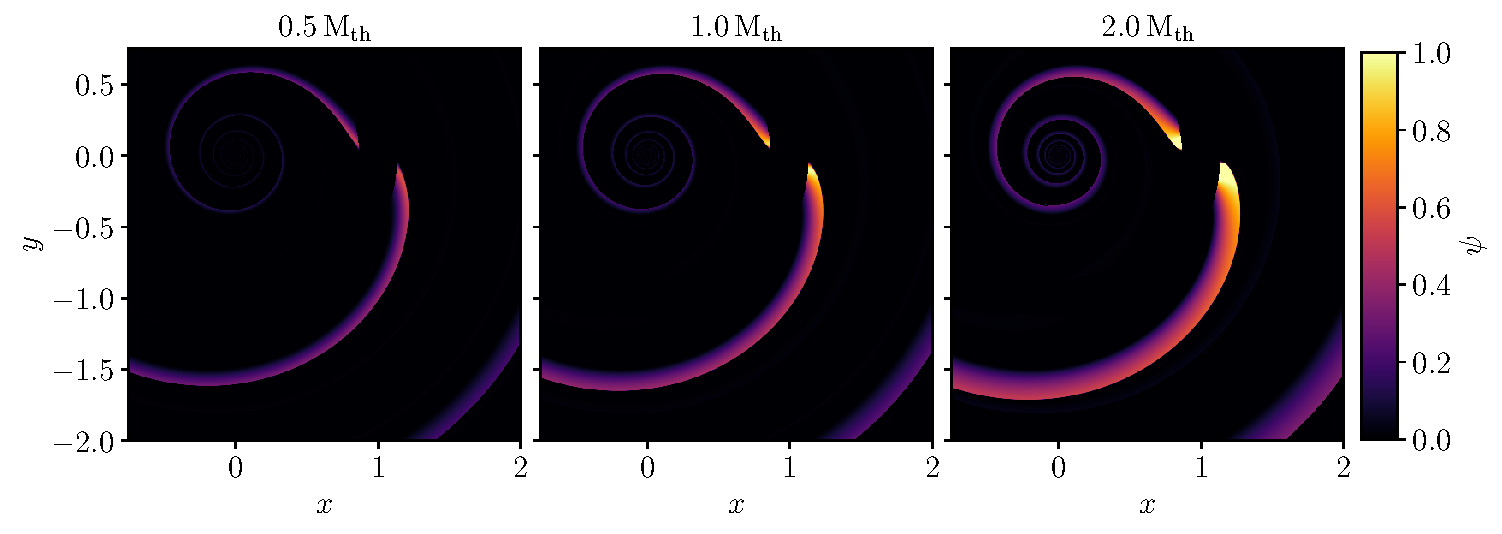
\includegraphics[width = 0.98\textwidth]{figures/psi 2.pdf}
    \caption{Comparison of the values of $\psi$ calculated from Equation \ref{eq:psi_exact} for three \textsc{wakeflow} models with planet masses of $0.5, 1.0$ and $2.0 \, M_{\rm{th}}$ respectively. Clearly one cannot assume that $\psi \ll 1$ even for the lowest mass model, especially nearby the planet. For the two larger masses, there are even regions where $\psi > 1$.}
    \label{fig:psi_comparison}
\end{figure}

To improve upon the velocity calculations used in \citet{bollati2021}, here we derive expressions for both $u$ and $v$ as functions of $\chi$ without truncating the equation of state to first order in $\psi$. This is as simple as substituting Equation \ref{eq:psi_exact} into Equations \ref{eq:u_rafikov} and \ref{eq:v_rafikov}, yielding
\begin{align}
    u(\chi) &= -2 \frac{c_0}{\gamma - 1} \left[ \left( \frac{2}{\gamma + 1} \frac{\chi}{g(r)} +1  \right)^{(\psi-1)/2} -1 \right] \\
    v(\chi) &\approx \frac{c_0}{\Delta\Omega r} u (\chi).
\end{align}




which are the expressions used to calculate the velocity perturbations in the non-linear regime in \textsc{wakeflow}. 

\begin{figure}
    \centering
    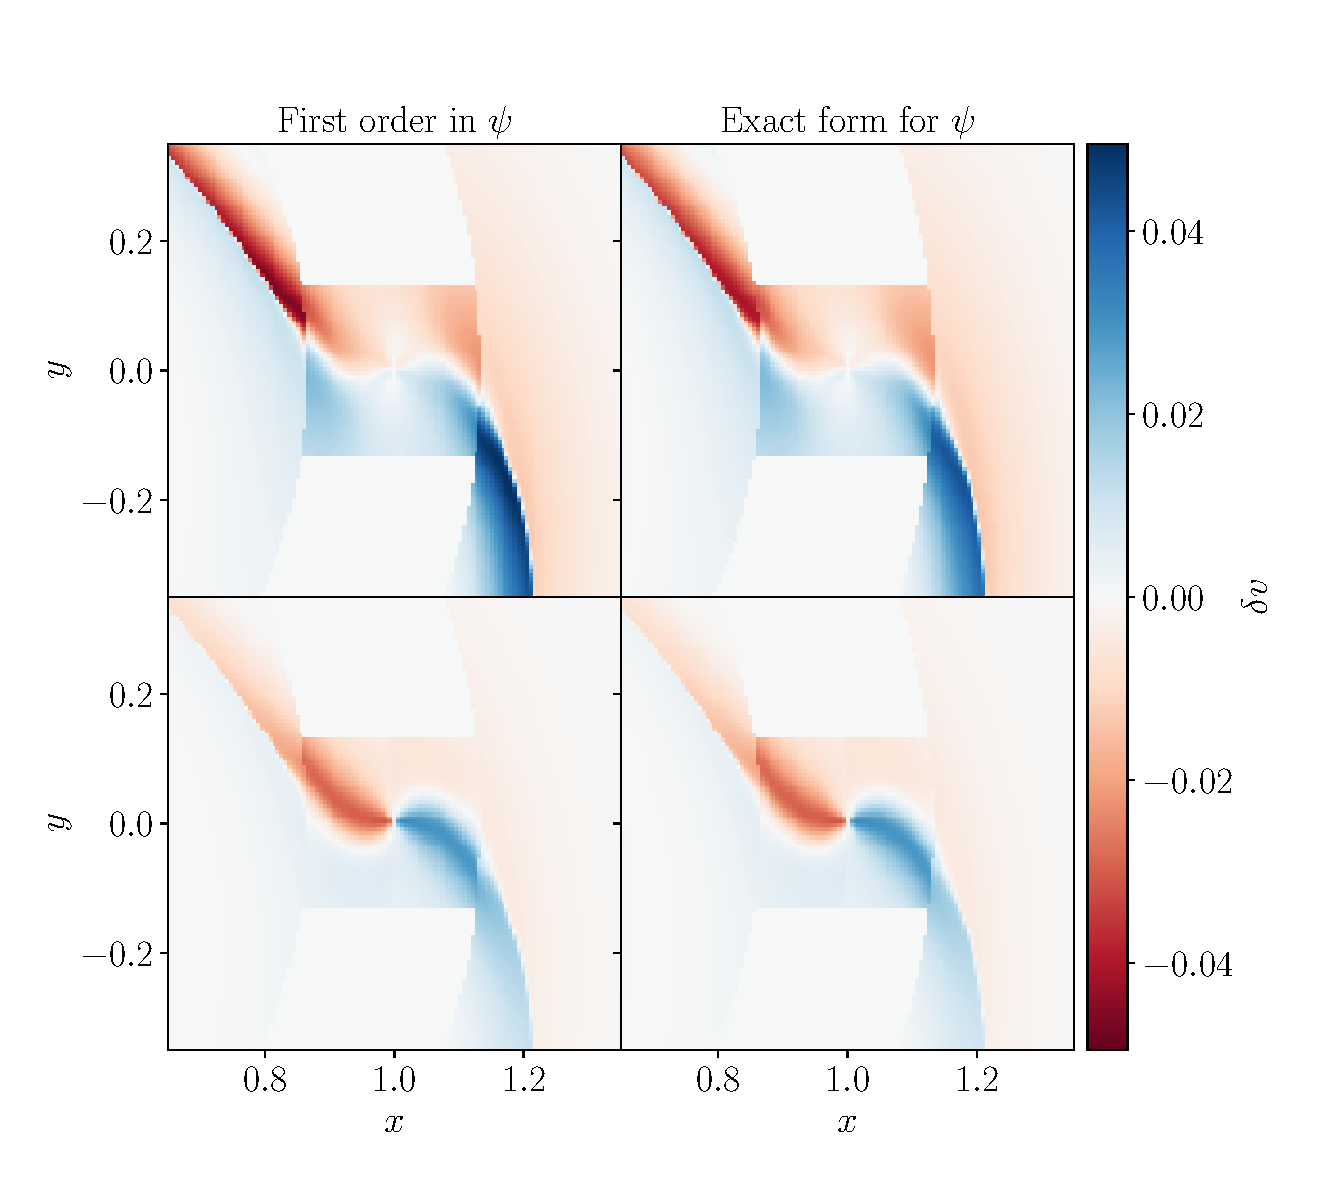
\includegraphics[width = 0.7\textwidth]{figures/0_5_mth.pdf}
    \caption{}
    \label{fig:0_5mth}
\end{figure}

\begin{figure}
    \centering
    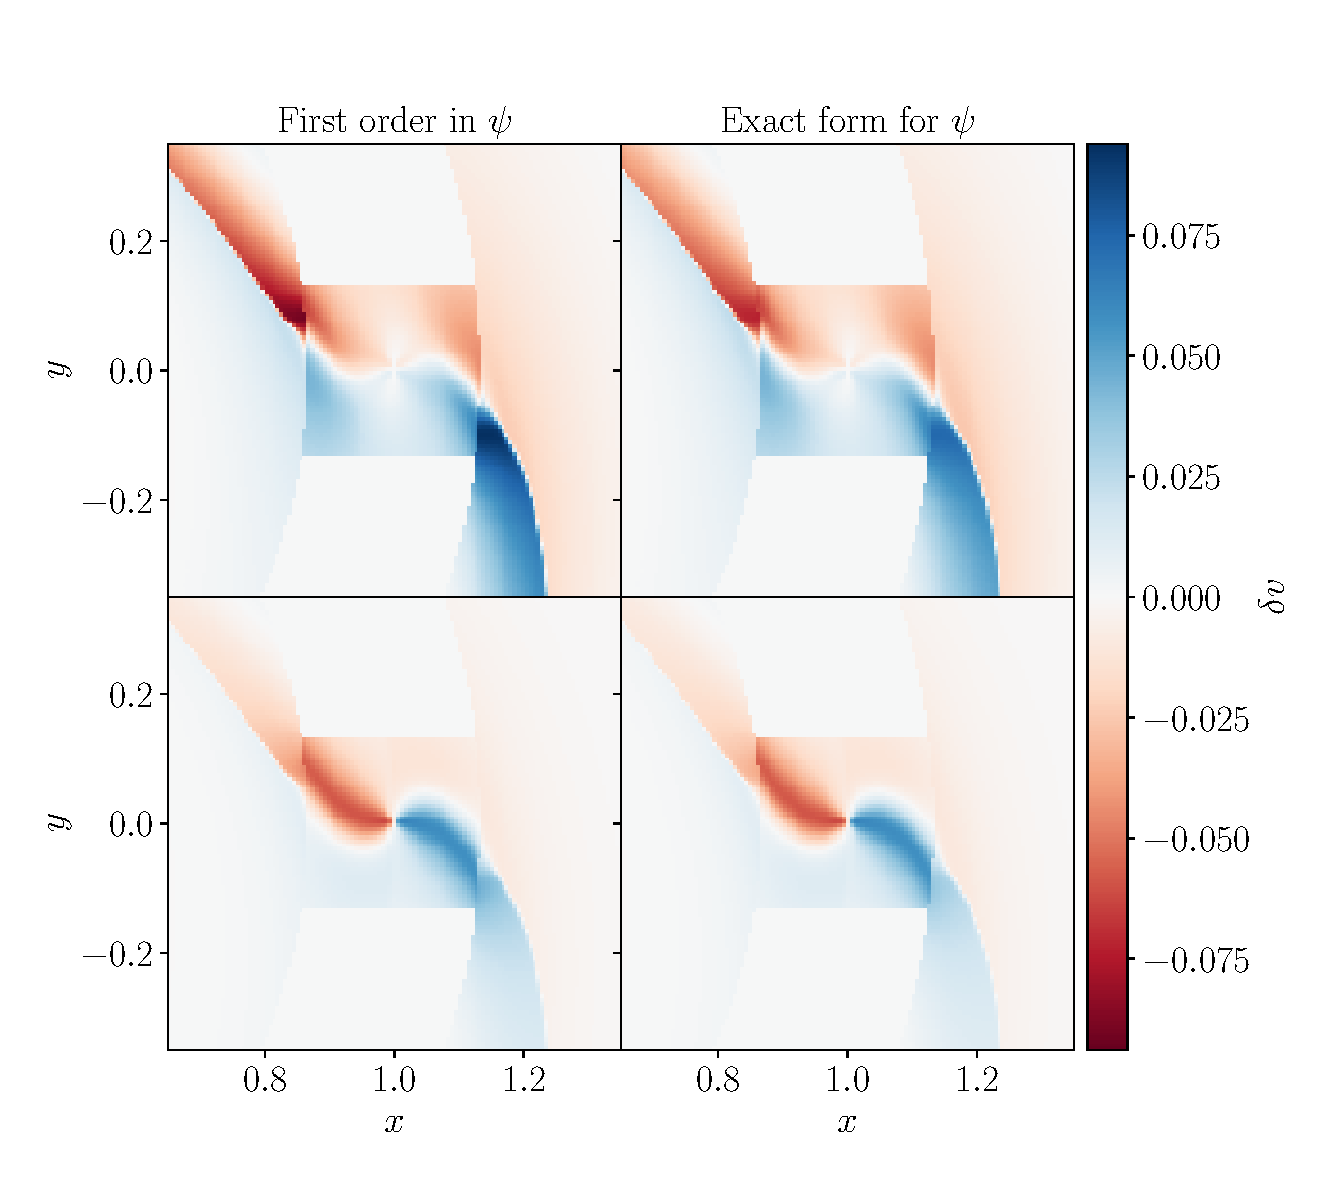
\includegraphics[width = 0.7\textwidth]{figures/1_0_mth.pdf}
    \caption{}
    \label{fig:1_0mth}
\end{figure}

\begin{figure}
    \centering
    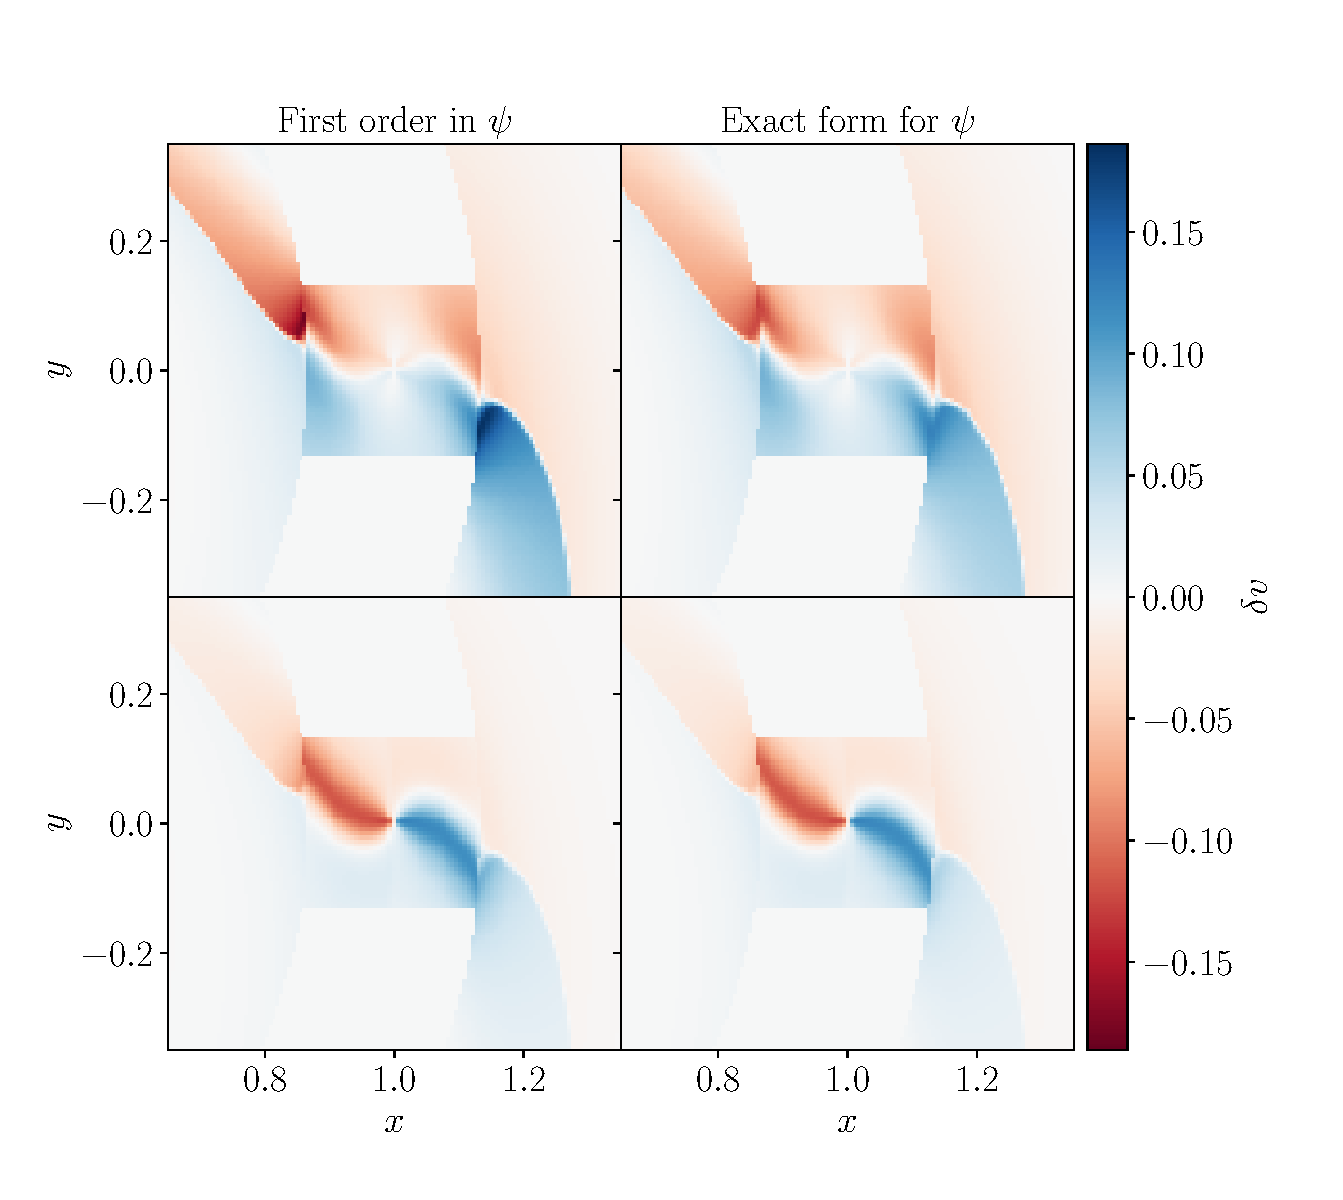
\includegraphics[width = 0.7\textwidth]{figures/2_0_mth.pdf}
    \caption{}
    \label{fig:2_0mth}
\end{figure}



\section{Synthetic Kinematic Observations}

\subsection{Predictions from 2D Models}

\subsection{3D Models}

\subsection{Radiation Transfer}